\section{Introduction}

When the data you want to model is high-dimensional, that is, the number of features \(p\)
exceed the number of observations \(n\), it is impossible to apply classical statistical
models such as standard linear regression since the design matrix \(\mat X\) is no longer
of full rank. A common remedy to this problem is to \emph{regularize} the model by adding a
term to the objective function that punishes models with large coefficients
(\(\vec\beta\)). If we let \(g(\vec\beta; \mat X, \vec y)\) be the original objective
function---which when minimized improves the model's fit to the data (\(\mat X, \vec
y\))---then
\[
  f(\beta_0, \vec\beta; \mat X, \vec y) = g(\beta_0, \vec\beta; \mat X, \vec y) + h(\vec\beta)
\]
is a composite function within which we have added a penalty term \(h(\vec\beta)\). In
contrast to \(g\), this penalty depends only on \(\vec{\beta}\). The intercept,
\(\beta_0\), is not typically penalized.

Some of the most common penalties are the \(\ell_1\) norm and squared \(\ell_2\) norm
penalties, that is \(h(\vec\beta) = \lVert \vec\beta \rVert_1\) or \(h(\vec\beta) = \lVert
\vec\beta \rVert_2^2/2\)\footnote{Division by two in this case is used only for
  convenience.}, which, if \(h\) is the standard ordinary least-squares objective, represent
lasso~\citep{tibshirani1996,santosa1986,donoho1994} and ridge (Tikhonov) regression
respectively. Other common penalities include SLOPE~\citep{bogdan2013,bogdan2015}, the
minimax-concave penalty (MCP)~\citep{zhang2010}, hinge loss (used in support vector
machines~\citep{cortes1995}) and smoothly-clipped absolute
deviation~(SCAD)~\citep{fan2001}. Many of these penalities---indeed all of the previously
mentioned ones---shrink coefficients in proportion to their sizes.

% TODO: Maybe say something about ℓ₀ (best subset) regularization
The issue with this type of shrinkage is that it is typically sensitive to the scales of
the features in \(\mat X\). A common remedy is to \emph{normalize} the features before
fitting the model by translating and dividing each column by respective translation and
scaling factors. For some problems, such factors may arise naturally from knowledge of the
problem at hand. A researcher may for instance have collected data on coordinates within a
limited area and know that the coordinates are measured in meters. Often, however, these
scaling factors must be estimated from data. The most popular choices for this type of
scaling are based only on the marginal distributions of the features. Some types of
normalization, such as that applied in the adaptive lasso\footnote{The adaptive lasso
  typically uses estimates of the regression coefficients, typically from ordinary-least
  squares or ridge regression, to scale the features with.}~\citep{zou2006}, however, are
based on the conditional distributions of the features and the response. After fitting the
model, the estimated coefficients are then usually returned to their original scale.
Another reason for normalizing the features is to improve the performance and stability of
optimization algorithms used to fit the model. We will not cover this aspect in this paper,
but note that it is an important one.

In most sources and discussions on regularized methods, normalization is typically treated
as a preprocessing step---separate from modeling. As we will show in this paper, however,
the type of normalization used can have a critical effect on the estimated model, sometimes
leading to entirely different conclusions with regard to feature importance as well as
predictive performance. As a first example of this, consider \Cref{fig:realdata-paths},
which displays the lasso paths for four real data sets and two different types of
normalization. Each panel shows the union of the first five predictors picked under either
normalization scheme. The choice of normalization can have a significant impact on the
estimated model. In the case of the \texttt{leukemia} data set, for instance, the models
are starkly different with respect to both the identities of the features selected as well
as their signs and magnitudes.

\begin{figure}[bpt]
  \centering
  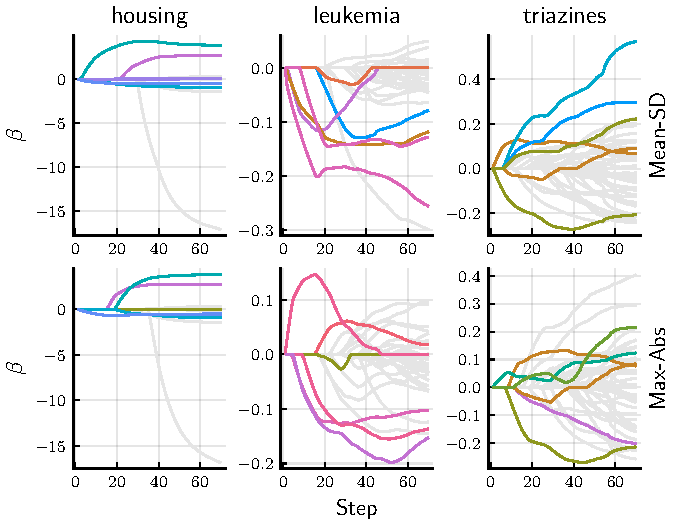
\includegraphics[]{plots/realdata_paths.pdf}
  \caption{%
    Lasso paths for real datasets using two types of normalization: standardization and maximum absolute value scaling (max--abs). We have fit the lasso path to four different datasets: \data{housing}~\citep{harrison1978}, \data{leukemia}~\citep{golub1999}, \data{triazines}~\citep{king}, and \data{w1a}~\citep{platt1998}. For each dataset, we have colored the coefficients if they were among the first five features to become active in under either of the two types of normalization schemes. We see that the paths differ with regards to the size as well as the signs of the coefficients, and that, in addition, the coefficients to become active first differ between the normalization types.
  }
  \label{fig:realdata-paths}
\end{figure}

In addition, discussions on the choice of normalization are often focused on computational
aspects and data storage requirements, rather than on the statistical properties of the
choice of normalization. In our paper, we argue that normalization should rather we
considered as an integral part of the model and that it is problematic to base the choice
of normalization on the type of data storage, which implicitly encodes the belief that the
information in a data set is different if it is stored in a sparse viz-a-viz dense format.
At the time of writing, for instance, the popular machine learning library
\texttt{scikit-learn}~\citep{scikit-learndevelopers2024} recommends max--abs scaling in the
case of sparse data.
